\chapter{Introduction}

\begin{center}
    \makebox[\textwidth]{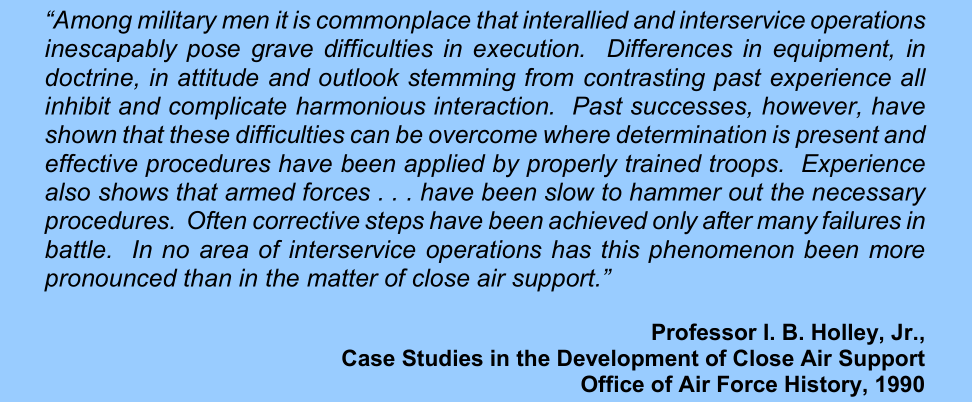
\includegraphics[width=\paperwidth]{quote1.png}}
\end{center}

\import{chapters/}{101-fundamentals}

\e
	
    \item 
	Bien que l'objectif principal du \gls{cas} soit de fournir un cadre de travail dans des conditions bien spécifiques, les techniques décrites dans ce manuel peuvent être appliquées à toute situation nécessitant un \gls{tac}.%
\ed

\section{Aperçu}

\e
    \item
    Le \gls{cas} est une action effectuée par des appareils à voilure fixe ou à voilure tournante contre des cibles ennemies \textbf{proches des forces amies} et nécessite une \textbf{coordination étroite} entre les missions de support aérien et le mouvement des troupes amies.
    \item
    Le \gls{cas} est planifié et exécuté pour appuyer les unités amies au sol. Le \gls{cas} est étroitement intégré au niveau du contrôle tactique des forces amies supportées. Alors que l'affectation des ressources aériennes disponibles se fait au niveau stratégique opérationnel, le processus de planification du \gls{cas} se fait au niveau stratégique local, pour fournir aux unités amies au contact de l'ennemi un appui-feu précis et rapide.
    \item
    Le \gls{cas} peut être effectué partout ou les forces amies se trouvent au contact de l'ennemi. Le mot ``rapproché'' (``Close'') n'implique pas une distance spécifique, mais plutôt un contexte. Parfois, le \gls{cas} peut être le meilleur moyen d'exploiter une opportunité tactique en défense ou en attaque. Le \gls{cas} fournit un appui-feu capable de détruire, perturber, interdire, empêcher, harceler, neutraliser ou retarder l'ennemi.
    \item
    Chaque organisation s'entraîne et emploie le \gls{cas} en tant que partie d'une coalition. Le \gls{jfc} est responsable d'intégrer ces organisations au \gls{conops} en fonctions de leurs capacités.
    \item
    Le \gls{tac} est l'autorité responsable de manœuvrer les appareils de soutien aérien et d'autoriser l'attaque finale. Un \gls{jtac} ou un \gls{faca} certifié sera reconnu comme capable et autorisé à effectuer le \gls{tac}.
    \item
    Il y a trois types de contrôle (type 1, 2 et 3):
    \ee
        \item
        Contrôle de \gls{typeone}

        Le contrôle de type 1 est utilisé lorsque le \gls{jtac}/\gls{faca} a besoin de contrôler de chaque attaque individuellement ainsi que d'avoir en permanence en visuel l'appareil qui attaque ainsi que sa cible.
        \item
        Contrôle de \gls{typetwo}

        Le contrôle de type 2 est utilisé lorsque le \gls{jtac}/\gls{faca} a besoin de contrôler chaque attaque mais qu'il ne peut pas voir l'appareil au moment du largage ou qu'il ne peut pas voir la cible.
        \item
        Contrôle de \gls{typethree}

        Le contrôle de \gls{typethree} est utilisé lorsque le \gls{jtac}/\gls{faca} a besoin de contrôler chaque engagement, avec ses restrictions, mais qu'on engagement peut être composé de plusieurs attaques.
    \ed
     \fullref{controltypessection}.
    \item \gls{tgo}: le personnel effectuant les \glspl{tgo} n'ont pas l'autorité pour contrôler les appareils engagés en opération \gls{cas} ou pour autoriser le tir.
\ed
    
\section{Usage du CAS}

\e
	\item
	L'usage du \gls{cas} s'inscrit dans le \gls{conops} de par sa spécificité à pouvoir frapper des cibles inaccessibles aux troupes au sol.
	
	\item
	Le \gls{gc} garde l'autorité suprême quant à l'usage d'armement dans sa zone de contrôle.
	
	\item
	Utilité sur le champ de bataille: le \gls{cas} permet au \gls{gc} de frapper l'ennemi rapidement et de manière inattendue.
	
	\item Critères pour l'usage du \gls{cas}:
	
	\ee
		\item Mission et \gls{conops}.
		\item Disposition, force et composition de l'ennemi.
		\item Capacités et limitations des appareils engagés dans le \gls{cas}.
		\item Emplacement et équipement des \gls{jtac}.
		\item \glspl{roe}.
		\item \gls{spins}.
		\item Défenses anti-aériennes ennemies et capacités alliées à les contrer.
		\item Disposition des forces amies
		\item Allocation des sorties \gls{cas}.
		\item Emplacement des civils et estimation des dommages collatéraux potentiels.	
	\ed
	
	\item Les cibles du \gls{cas} sont sélectionnées par le \gls{jtac}, en fonction des intentions du \gls{gc}, du terrain, de la météo, de la mission, des défenses ennemies, de l'armement disponible, du temps de réponse, etc. D'autres considérations peuvent entrer en ligne de compte.
\ed
	
\section{Intégration du CAS}
\e
	\item Lors des opération conjointes, l'intégration du \gls{cas} commence au niveau opérationnel. S'il est établi, le \gls{jfacc} fournit ses recommandations au \gls{jfc}. Chaque composante informe le \gls{jfc} de ses besoins et limitations. Le \gls{jfc} implémente le cadre dans lequel les opérations d'interdiction (\gls{cas}, \gls{ai}, etc.) s'intégreront dans l'\gls{opord}, l'\gls{aod}, l'\gls{ato}, l'\gls{aco} et les \gls{spins}.
\ed

\section{Emploi des voilures fixes et des voilures tournantes en opérations de CAS}

\e
	\item
	La structure organisationnelle, la mission principale et les capacités des appareils capables d'effectuer le \gls{cas} déterminent leur emploi. Bien que les \glspl{fw} et les \glspl{rw} puissent tous deux effectuer le \gls{cas}, leur emploi diffère.
	
	\item
	De par leur vitesse et leur portée opérationnelle, les \glspl{fw} offrent une grande versatilité et une grande flexibilité. De plus, ils emploient un arsenal de munitions très varié, qui peut être employé par presque toutes les conditions (météo, luminosité, ...).
	
	\item
	Les \glspl{rw} permettent de manœuvrer et de repositionner rapidement la puissance de feu en fonction de l'évolution de la situation. Ils ont un excellent temps de réponse et peuvent rester longtemps sur zone, peuvent évoluer à très faible altitude, et peuvent effectuer du \gls{cas} sur tous les types de terrain. Ils offrent également des capacités d'infiltration et d'extraction du personnel.

\ed

\section{Efficacité du CAS}

\e
	\item 
	Pour que le \gls{cas} soit efficace, il faut:
	\ee
		\item Du personnel correctement entraîné \\
		L'entraînement au \gls{cas} doit intégrer toutes les manoeuvres et procédures nécessaires à l'exécution du \gls{cas}. Cet entraînement doit être tenu à jour.
		\item Un planning et une intégration réfléchie \\
		Un \gls{cas} efficace s'appuie sur une planification en profondeur. La capacité à fournir la puissance de feu nécessaire au bon endroit est possible de par l'intégration avec les forces au sol. De point de vue du planificateur, le \gls{cas} pré-planifié sera toujours préféré.
		\item Un \gls{cc} efficace \\
		Le \gls{cas} nécessite une structure \gls{cc} flexible et intégrée au reste du dispositif pour trier les demandes, assigner les priorités, assigner les tâches, repositionner les éléments, fournir les alertes de menaces, et augmenter les capacité de \gls{cid}.
		\item Une supériorité aérienne établie (tout particulièrement le \gls{sead})
		\item Une reconnaissance et une connaissance des cibles
		\item Des procédures flexibles et éprouvées
		\eee
			\item Placement des unités de \gls{cas} proche de leur zone d'opération. Placement des points d'attente de d'orbite de manière optimiser le temps de réaction.
			\item Délégation des autorisations de tir aux unités subordonnées.
			\item Ré-assignation des appareils en fonction des situations émergentes.
			\item Révision de l'\gls{ato} en fonction des situations émergents.
			\item Redirection des appareils \gls{cas} en réponse aux menaces.
			\item Délégation des autorité au plus bas niveau tactique possible.
			\item Placement des \gls{jtac} avec les unités au sol de manière à faciliter les communications et la coordination avec les appareils de \gls{cas}.			
		\ed
		\item De l'armement approprié \\
		Le \gls{gc} et le \gls{jtac} doivent connaître l'effet de l'armement employé, de manière à pouvoir évaluer les possibilités de dommages collatéraux, et l'impact sur le poursuite de la mission.
		\item Des conditions environnementales \\
		Des conditions favorables améliorent l'efficacité des unités de \gls{cas} quelles que soient les capacités de l'appareil ou de l'armement. \textbf{Avant d'envisager une mission de \gls{cas}, des conditions météo minimales doivent être définies}. Certaines conditions peuvent n'influencer que certaines plateformes; par exemple, un plafond très bas peut rendre certains \glspl{fw} inutiles, sans impacter les \glspl{rw}. Inversement, les \glspl{fw} pourront opérer lors d'une tempête de sable qui clouerait les \glspl{rw} au sol. Les conditions météo influencent également fortement le marquage de la cible.	
		
	\ed
\ed

\section{Responsabilités}

\e
	\item \gls{jfc} \\
	Le \gls{jfc} établit le cadre et les priorités pour le \gls{cas} dans le \gls{conops}.
	
	\item \gls{jfacc} \\
	Le \gls{jfacc} reçoit du \gls{jfc} l'autorité pour créer des missions et des tâches.
	
	\item \note{Le commandant d'escadron s'assure que ses unités sont capables d'exécuter des missions de \gls{cas}}
\ed
	
\section{Minimiser le tir fratricide}

\e
	\item Le tir fratricide est parfois le résultat tragique de la guerre.
	\item
	\textbf{Bien que parfois le résultat d'armement défectueux, le tir fratricide est souvent le résultat de la confusion qui règne sur le champ de bataille.}
	\note {Kakane, celle-là est pour toi !}
	Les causes peuvent être, entre autres:
	\ee
		\item Mauvaise identification de la cible
		\item Position ou description de la cible erronée
		\item Mauvaise transmission de la position ou de la description de la cible
		\item Perte de \gls{sa} par le pilote ou le \gls{jtac}
	\ed
	\item Responsabilités \\
	Tout le personnel impliqué dans le \gls{cas} est responsable de la sécurité lors du planning et de l'exécution. Chaque participant doit tout entreprendre pour identifier les unités alliées, les forces ennemies et les civils avant de prendre pour cible, d'engager, ou d'autoriser le tir.
	\item Entraînement \\
	La coalition, ses composantes, et les unités doivent effectuer un entraînement conjoint régulier qui simule des opérations réelles de manière à développer les capacités nécessaires au bon déroulement du \gls{cas}.	
\ed

\section{Minimiser les victimes civiles}
\e
	\item Les lois de la guerre obligent tous les commandants à prendre toutes les précautions nécessaires pour minimiser les victimes civiles et les dégâts collatéraux.
\ed
